\documentclass{extbook}[14pt]
\usepackage{multicol, enumerate, enumitem, hyperref, color, soul, setspace, parskip, fancyhdr, amssymb, amsthm, amsmath, latexsym, units, mathtools}
\everymath{\displaystyle}
\usepackage[headsep=0.5cm,headheight=0cm, left=1 in,right= 1 in,top= 1 in,bottom= 1 in]{geometry}
\usepackage{dashrule}  % Package to use the command below to create lines between items
\newcommand{\litem}[1]{\item #1

\rule{\textwidth}{0.4pt}}
\pagestyle{fancy}
\lhead{}
\chead{Answer Key for Module6 Version A}
\rhead{}
\lfoot{7334-5530}
\cfoot{}
\rfoot{test}
\begin{document}
\textbf{This key should allow you to understand why you choose the option you did (beyond just getting a question right or wrong). \href{https://xronos.clas.ufl.edu/mac1105spring2020/courseDescriptionAndMisc/Exams/LearningFromResults}{More instructions on how to use this key can be found here}.}

\textbf{If you have a suggestion to make the keys better, \href{https://forms.gle/CZkbZmPbC9XALEE88}{please fill out the short survey here}.}

\textit{Note: This key is auto-generated and may contain issues and/or errors. The keys are reviewed after each exam to ensure grading is done accurately. If there are issues (like duplicate options), they are noted in the offline gradebook. The keys are a work-in-progress to give students as many resources to improve as possible.}

\rule{\textwidth}{0.4pt}

\begin{enumerate}\litem{
Describe the zero behavior of the zero $x = 7$ of the polynomial below.
\[ f(x) = 7(x + 2)^{12}(x - 2)^{8}(x + 7)^{12}(x - 7)^{9} \]The solution is the graph below.
    \begin{center}
        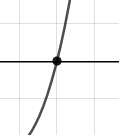
\includegraphics[width=0.3\textwidth]{../Figures/polyZeroBehaviorDA.png}
    \end{center}

\textbf{General Comment:} You will need to sketch the entire graph, then zoom in on the zero the question asks about.
}
\litem{
Write an equation that \textit{could} represent the graph below.

\begin{center}
    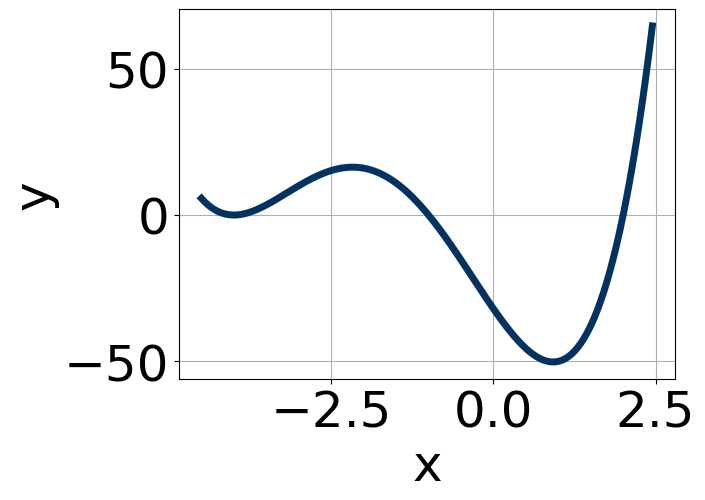
\includegraphics[width=0.5\textwidth]{../Figures/polyGraphToFunctionA.png}
\end{center}


The solution is \( -19(x + 1)^{5} (x - 2)^{9} (x + 3)^{5} \).\begin{enumerate}[label=\Alph*.]
\textbf{Plausible alternative answers include:}The factor $(x + 1)$ should have an odd power and the leading coefficient should be the opposite sign.
The factor $-1$ should have been an odd power.
The factors $-1$ and $2$ have have been odd power.
* This is the correct option.
This corresponds to the leading coefficient being the opposite value than it should be.
\end{enumerate}

\textbf{General Comment:} General Comments: Draw the x-axis to determine which zeros are touching (and so have even multiplicity) or cross (and have odd multiplicity).
}
\litem{
Construct the lowest-degree polynomial given the zeros below.
\[ -4, \frac{-2}{5}, \text{ and } \frac{-5}{3} \]The solution is \( 15x^{3} +91 x^{2} +134 x + 40 \).\begin{enumerate}[label=\Alph*.]
\textbf{Plausible alternative answers include:}* $15x^{3} +91 x^{2} +134 x + 40$, which is the correct option.
$15x^{3} -41 x^{2} -86 x + 40$, which corresponds to multiplying out $(x -4)(5x -2)(3x + 5)$.
$15x^{3} -91 x^{2} +134 x -40$, which corresponds to multiplying out $(x -4)(5x -2)(3x -5)$.
$15x^{3} +91 x^{2} +134 x -40$, which corresponds to multiplying everything correctly except the constant term.
$15x^{3} -29 x^{2} -114 x -40$, which corresponds to multiplying out $(x -4)(5x + 2)(3x + 5)$.
\end{enumerate}

\textbf{General Comment:} To construct the lowest-degree polynomial, you want to multiply out $(x + 4)(5x + 2)(3x + 5)$
}
\litem{
Describe the zero behavior of the zero $x = -3$ of the polynomial below.
\[ f(x) = -3(x - 2)^{7}(x + 2)^{6}(x + 3)^{7}(x - 3)^{4} \]The solution is the graph below.
    \begin{center}
        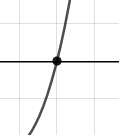
\includegraphics[width=0.3\textwidth]{../Figures/polyZeroBehaviorCopyDA.png}
    \end{center}

\textbf{General Comment:} You will need to sketch the entire graph, then zoom in on the zero the question asks about.
}
\litem{
Construct the lowest-degree polynomial given the zeros below.
\[ \frac{4}{3}, \frac{-7}{2}, \text{ and } \frac{6}{5} \]The solution is \( 30x^{3} +29 x^{2} -218 x + 168 \).\begin{enumerate}[label=\Alph*.]
\textbf{Plausible alternative answers include:}$30x^{3} +109 x^{2} -34 x -168$, which corresponds to multiplying out $(3x + 4)(2x + 7)(5x -6)$.
$30x^{3} +29 x^{2} -218 x -168$, which corresponds to multiplying everything correctly except the constant term.
$30x^{3} -101 x^{2} -62 x + 168$, which corresponds to multiplying out $(3x + 4)(2x -7)(5x -6)$.
* $30x^{3} +29 x^{2} -218 x + 168$, which is the correct option.
$30x^{3} -29 x^{2} -218 x -168$, which corresponds to multiplying out $(3x + 4)(2x -7)(5x + 6)$.
\end{enumerate}

\textbf{General Comment:} To construct the lowest-degree polynomial, you want to multiply out $(3x -4)(2x + 7)(5x -6)$
}
\litem{
Describe the end behavior of the polynomial below.
\[ f(x) = -3(x - 2)^{3}(x + 2)^{4}(x + 8)^{5}(x - 8)^{5} \]The solution is the graph below.
    \begin{center}
        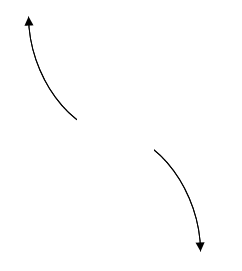
\includegraphics[width=0.3\textwidth]{../Figures/polyEndBehaviorCopyAA.png}
    \end{center}

\textbf{General Comment:} Remember that end behavior is determined by the leading coefficient AND whether the \textbf{sum} of the multiplicities is positive or negative.
}
\litem{
Construct the lowest-degree polynomial given the zeros below.
\[ 5 - 3 i \text{ and } -1 \]The solution is \( x^{3} -9 x^{2} +24 x + 34 \).\begin{enumerate}[label=\Alph*.]
\textbf{Plausible alternative answers include:}$x^{3} + x^{2} +4 x + 3$, which corresponds to multiplying out $(x + 3)(x + 1)$.
$x^{3} +9 x^{2} +24 x -34$, which corresponds to multiplying out $(x-(5 - 3 i))(x-(5 + 3 i))(x -1)$.
$x^{3} + x^{2} -4 x -5$, which corresponds to multiplying out $(x -5)(x + 1)$.
* $x^{3} -9 x^{2} +24 x + 34$, which is the correct option.
This corresponds to making an unanticipated error or not understanding how to use nonreal complex numbers to create the lowest-degree polynomial. If you chose this and are not sure what you did wrong, please contact the coordinator for help.
\end{enumerate}

\textbf{General Comment:} Remember that the conjugate of $a+bi$ is $a-bi$. Since these zeros always come in pairs, we need to multiply out $(x-(5 - 3 i))(x-(5 + 3 i))(x-(-1))$.
}
\litem{
Write an equation that \textit{could} represent the graph below.

\begin{center}
    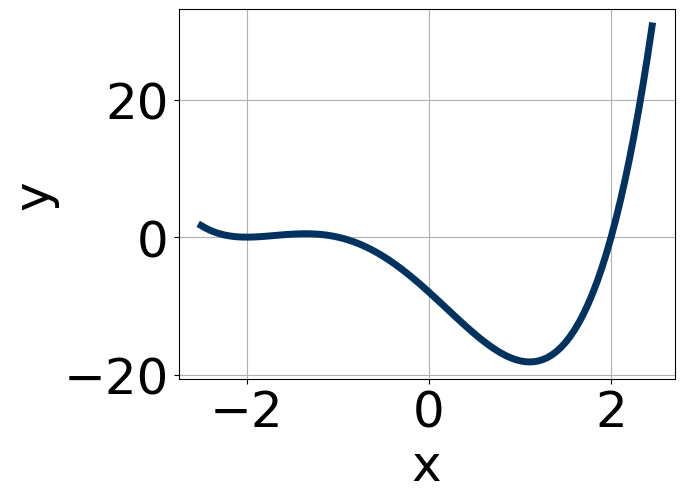
\includegraphics[width=0.5\textwidth]{../Figures/polyGraphToFunctionCopyA.png}
\end{center}


The solution is \( 20(x + 2)^{6} (x + 1)^{11} (x - 2)^{7} \).\begin{enumerate}[label=\Alph*.]
\textbf{Plausible alternative answers include:}The factor $-2$ should have an even power and the factor $-1$ should have an odd power.
* This is the correct option.
This corresponds to the leading coefficient being the opposite value than it should be.
The factor $(x - 2)$ should have an odd power and the leading coefficient should be the opposite sign.
The factor $(x + 1)$ should have an odd power.
\end{enumerate}

\textbf{General Comment:} General Comments: Draw the x-axis to determine which zeros are touching (and so have even multiplicity) or cross (and have odd multiplicity).
}
\litem{
Construct the lowest-degree polynomial given the zeros below.
\[ -5 + 3 i \text{ and } -2 \]The solution is \( x^{3} +12 x^{2} +54 x + 68 \).\begin{enumerate}[label=\Alph*.]
\textbf{Plausible alternative answers include:}$x^{3} + x^{2} -x -6$, which corresponds to multiplying out $(x -3)(x + 2)$.
* $x^{3} +12 x^{2} +54 x + 68$, which is the correct option.
$x^{3} + x^{2} +7 x + 10$, which corresponds to multiplying out $(x + 5)(x + 2)$.
$x^{3} -12 x^{2} +54 x -68$, which corresponds to multiplying out $(x-(-5 + 3 i))(x-(-5 - 3 i))(x -2)$.
This corresponds to making an unanticipated error or not understanding how to use nonreal complex numbers to create the lowest-degree polynomial. If you chose this and are not sure what you did wrong, please contact the coordinator for help.
\end{enumerate}

\textbf{General Comment:} Remember that the conjugate of $a+bi$ is $a-bi$. Since these zeros always come in pairs, we need to multiply out $(x-(-5 + 3 i))(x-(-5 - 3 i))(x-(-2))$.
}
\litem{
Describe the end behavior of the polynomial below.
\[ f(x) = 5(x + 8)^{5}(x - 8)^{10}(x + 3)^{5}(x - 3)^{5} \]The solution is the graph below.
    \begin{center}
        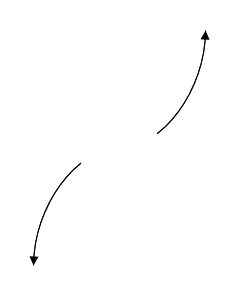
\includegraphics[width=0.3\textwidth]{../Figures/polyEndBehaviorDA.png}
    \end{center}

\textbf{General Comment:} Remember that end behavior is determined by the leading coefficient AND whether the \textbf{sum} of the multiplicities is positive or negative.
}
\end{enumerate}

\end{document}